	\newpage
\section{Rozpoznanie wzorców projektowych}		%9
\textbf{\textit{a) Metoda szablonowa}} - to wzorzec projektowy definiujący szkielet algorytmu w klasie bazowej. Pozwala podklasom nadpisać pewne etapy algorytmu bez konieczności zmiany ich struktury.
\\Rozwiązanie zawarte we wzorcu Metody szablonowej zakłada rozdzielenie algorytmu na kolejne etapy, utworzenie z tych etapów metod i umieszczenie ciągu wywołań poszczególnych metod w jednej metodzie szablonowej. Etapy mogą być albo abstrakcyjne, albo posiadać jakąś domyślną implementację. Aby skorzystać z algorytmu, klient powinien dostarczyć swoją podklasę implementującą wszystkie etapy abstrakcyjne i nadpisać opcjonalne etapy jeśli jest taka potrzeba (oprócz samej metody szablonowej).
\newline\textbf{\textit{b) Budowniczy}} - jest kreacyjnym wzorcem projektowym, który daje możliwość tworzenia złożonych obiektów etapami, krok po kroku. Wzorzec ten pozwala produkować różne typy oraz reprezentacje obiektu używając tego samego kodu konstrukcyjnego. Wzorzec ten proponuje ekstrakcję kodu konstrukcyjnego obiektu z jego klasy i umieszczenie go w osobnych obiektach zwanych budowniczymi. Dzieli on konstrukcję obiektu na pewne etapy. Aby powołać do życia obiekt, wykonuje się ciąg takich etapów za pośrednictwem obiektu-budowniczego. Istotne jest to, że nie trzeba wywoływać wszystkich etapów naraz. Można bowiem ograniczyć się tylko do tych kroków, które są niezbędne do określenia potrzebnej nam konfiguracji obiektu na dany moment.
\newline\textbf{\textit{c) Adapter}} - jest strukturalnym wzorcem projektowym pozwalającym na współdziałanie ze sobą obiektów o niekompatybilnych interfejsach. Jest to specjalny obiekt konwertujący interfejs jednego z obiektów w taki sposób, że drugi obiekt go rozumie.
\\Adapter stanowi swego rodzaju opakowanie dla obiektu, ukrywając szczegóły konwersji jakie odbywają się za kulisami. Obiekt opakowywany może nawet nie wiedzieć o istnieniu adaptera. Można na przykład opakować obiekt korzystający z jednostek kilometr i metr w adapter konwertujący te dane na jednostki imperialne, takie jak stopy i mile.
Adaptery mogą nie tylko konwertować dane pomiędzy formatami, ale również pozwolić na współpracę obiektów o różnych interfejsach. Działa to tak:
\\Adapter uzyskuje interfejs kompatybilny z interfejsem jednego z obiektów.
Następnie za pomocą tego interfejsu, istniejący obiekt może śmiało wywoływać metody adaptera.
Otrzymawszy wywołanie, adapter przekazuje je dalej, ale już w formacie obsługiwanym przez opakowany obiekt.
\\Czasami jest nawet możliwe stworzenie adaptera dwukierunkowego, potrafiącego konwertować wywołania w obu kierunkach.
\newline\textbf{\textit{d) Singleton}} - jest kreacyjnym wzorcem projektowym, który pozwala zapewnić istnienie wyłącznie jednej instancji danej klasy. Ponadto daje globalny punkt dostępowy do tejże instancji. Singleton rozwiązuje jednocześnie dwa problemy. Po pierwsze zapewnia istnienie wyłącznie jednej instancji danej klasy, a po drugie pozwala na dostęp do tej instancji w przestrzeni globalnej.
\\Wszystkie implementacje wzorca Singleton współdzielą poniższe dwa etapy:
\\Ograniczenie dostępu do domyślnego konstruktora przez uczynienie go prywatnym, aby zapobiec stosowaniu operatora new w stosunku do klasy Singleton.
\\Utworzenie statycznej metody kreacyjnej, która będzie pełniła rolę konstruktora. Za kulisami, metoda ta wywoła prywatny konstruktor, aby utworzyć instancję obiektu i umieści go w polu statycznym klasy. Wszystkie kolejne wywołania tej metody zwrócą już istniejący obiekt.
\newline\textbf{\textit{e) Odwiedzający}} - to behawioralny wzorzec projektowy pozwalający oddzielić algorytmy od obiektów na których pracują.
\\Wzorzec projektowy Odwiedzający proponuje umieszczenie nowych obowiązków w osobnej klasie zwanej odwiedzającym, zamiast próbować zintegrować je z istniejącymi klasami. Pierwotny obiekt, który miał wykonywać te obowiązki, teraz jest przekazywany do jednej z metod odwiedzającego w charakterze argumentu. Daje to metodzie dostęp do wszystkich potrzebnych danych znajdujących się w obiekcie.
\newline\textbf{\textit{f) Dekorator}} - umożliwia dynamiczne przydzielenie wybranemu obiektowi nowych zachowań. Dekoratory dają elastyczność podobną do tej, jaką daje dziedziczenie, jednak oferują znacznie lepszą funkcjonalność.
\newline\textbf{\textit{g) Fasada}} - należy do wzorców strukturalnych. W tym wzorcu jedna klasa nadrzędna zawiera mniejsze obiekty klas, którymi zarządza udostępniając użytkownikowi (programowi) zewnętrznemu odpowiednie metody upraszczające obsługę działań na obiektach weń znajdujących się.
\newline\textbf{\textit{g) Kompozyt}} - umożliwia on tworzenie struktur drzewiastych, gdzie podstawową jednostką jest liść  a rozszerzoną kompozyt, przy czym kompozyt można opisać jako swego rodzaju gałąź struktury. Oba te elementy (liść i kompozyt) dziedziczą po wspólnym interfejsie. Sam kompozyt zawiera kontener, który może przechowywać interfejsy, za którymi mogą stać jednostki podstawowe (liście) lub kolejne gałęzie (kompozyty).
\newline\textbf{\textit{h) Obserwator}} - jego celem jest wywoływanie klasy zawierającej klasy obserwatorów w momencie, gdy zajdzie określona zmiana w obiekcie obserwowanym. Innymi słowy jeżeli obserwowany obiekt zmienia stan, wtedy uruchamia on odpowiednią metodę klasy zawierającej obserwatorów a ta wywołuje kolejno metody na zarejestrowanych obserwatorach.
\newline\newline W naszym projekcie został użyty wzorzec projektowy o nazwie bloc. Jest to bardzo popularny wzorzec w środowisku programistycznym flutter i jest często wykorzystywany przez duże korporacje. Wzorzec bloc służy do oddzielenia warstwy logicznej - backendu od warstwy biznesowej - UI/layout. Bloc pozwala na wygodne ustrukturyzowanie plików w projekcie, tak aby wiele osób mogło pracować skutecznie w ramach jednego projektu. Bloc również rozwiązuje wiele podstawowych problemów związanych z state managment, co pozwala na zarządzaniu stanami za pośrednictwem innych klas. Bloc zwykle składa się z modeli, czyli klas na których będziemy operować, view czyli widoków dla poszczególnych bloków, eventów, czyli akcji, które będą wywoływały jakieś akcje np. zmiany stanów oraz stany jakie może przyjmować dany blok. We flutterze aby bloc działał poprawnie, należy zaimportować paczkę bloc oraz użyć blocbuilder'a, aby przechodzić pomiędzy 
stanami wywołując dane widoki za pomocą eventów.

%rysunek
\begin{figure}[!htb]
	\begin{center}
		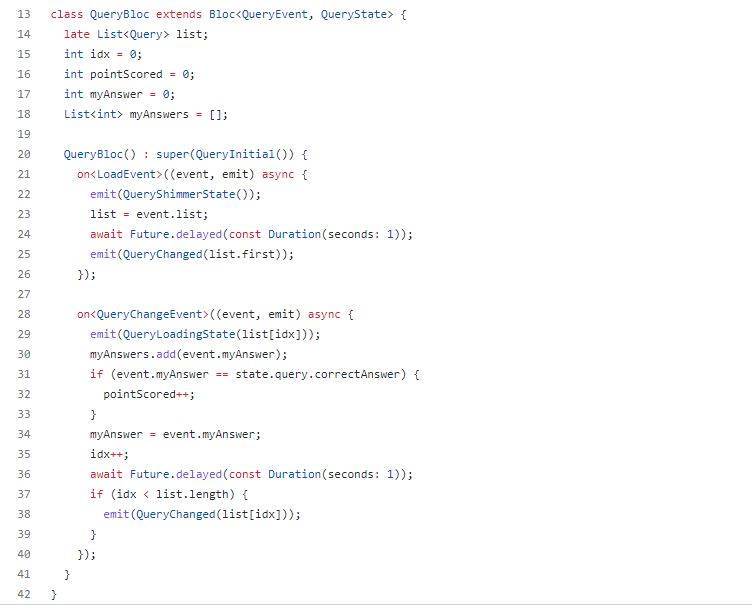
\includegraphics[width=15cm]{rys/bloc1.png}
		\caption{Bloc - implementacja}
		\label{rys:rysunek004}
	\end{center}
\end{figure} 
